\newpage
\chapter{Model Design and Development}\label{sec:model}
\subsubsection{Background}
Model-based methods for controlling the arm as a unified system and determining real-world arm dynamics have been suggested in earlier studies as a solution for precise control. For instance, physics-based models have demonstrated some success in controlling two muscles for rehabilitation \cite{IOL}. However, a major challenge lies in the identification of the physical parameters of the entire arm, which demands a significant amount of data.

To address this issue, black-box model-based control methods have been developed. An example of these methods successfully utilized an artificial neural network (ANN) to create a map of task space configuration in relation to the forces that muscles can generate, thereby achieving control of planar arm tasks \cite{FC2D}. Moreover, Lyapunov-based methods have been employed to create a data-driven Deep Neural Network (DNN) based adaptive control method used for Functional Electrical Stimulation (FES)-induced leg extension rehabilitation \cite{CLDNN}.

Another difficulty lies in establishing control parameters for these systems, with new parameters needing to be set for each subject. Even for the same subject, these parameters can vary under different conditions, making the traditional control theory that requires a mathematical model of the controlled system unsuitable \cite{NNPID}. 

Despite the potential of model-based FES control in providing necessary accuracy, few approaches have found their way into clinical practice. This shortfall can be attributed to challenges in deriving an accurate model given the limited identification time due to factors such as onset of fatigue and time constraints of the patient, carer, physiotherapist, or engineer \cite{IOL}. Furthermore, due to time-varying physiological effects, models must be re-identified at the commencement of each treatment session.

Previous work has demonstrated that a semi-parametric Gaussian Process Regression (GPR) model can form the foundation for a controller achieving three-dimensional dynamic trajectories. This model-based method \cite{QSC} circumvents parametric modelling challenges owing to the difficulty in defining the parameters. The semiparametric GPR combines the generalization potential of a parameterized model with the ability of a nonlinear function approximator that represents the diversity of the musculoskeletal dynamics. 

In this project, we developed our model identification in a manner akin to the approach outlined in the paper \cite{QSC}, as it was found to be successful in circumventing the challenges intrinsic to parametric modeling. The GPR model provides a non-parametric, data-driven approach, allowing for an analytical representation of complex patterns without necessitating rigid assumptions regarding the model's structure.

\newpage
\subsubsection{Design}

 A two part modeled is developed consisting of:

 \begin{itemize}
     \item \textbf{Inverse Statics}. It calculates the joint torque needed to hold a desired static arm configuration.
     \item \textbf{Muscle Torque Production}. It maps the arm configuration with the muscle activation to the joint torque produced. 
 \end{itemize}

To gather data for the models a PI controller is designed to compute the force applied at the wrist in order to hold the arm in a static position, both with and without neural excitation. This force is subsequently converted into torque using the kinematic Jacobian. The process is detailed in sections \ref{sec:tp}, \ref{sec:PI} and \ref{sec:torque} and a flow diagram is shown in Figure \ref{fig:datacreation}. 

\begin{figure}[h!]
    \centering
    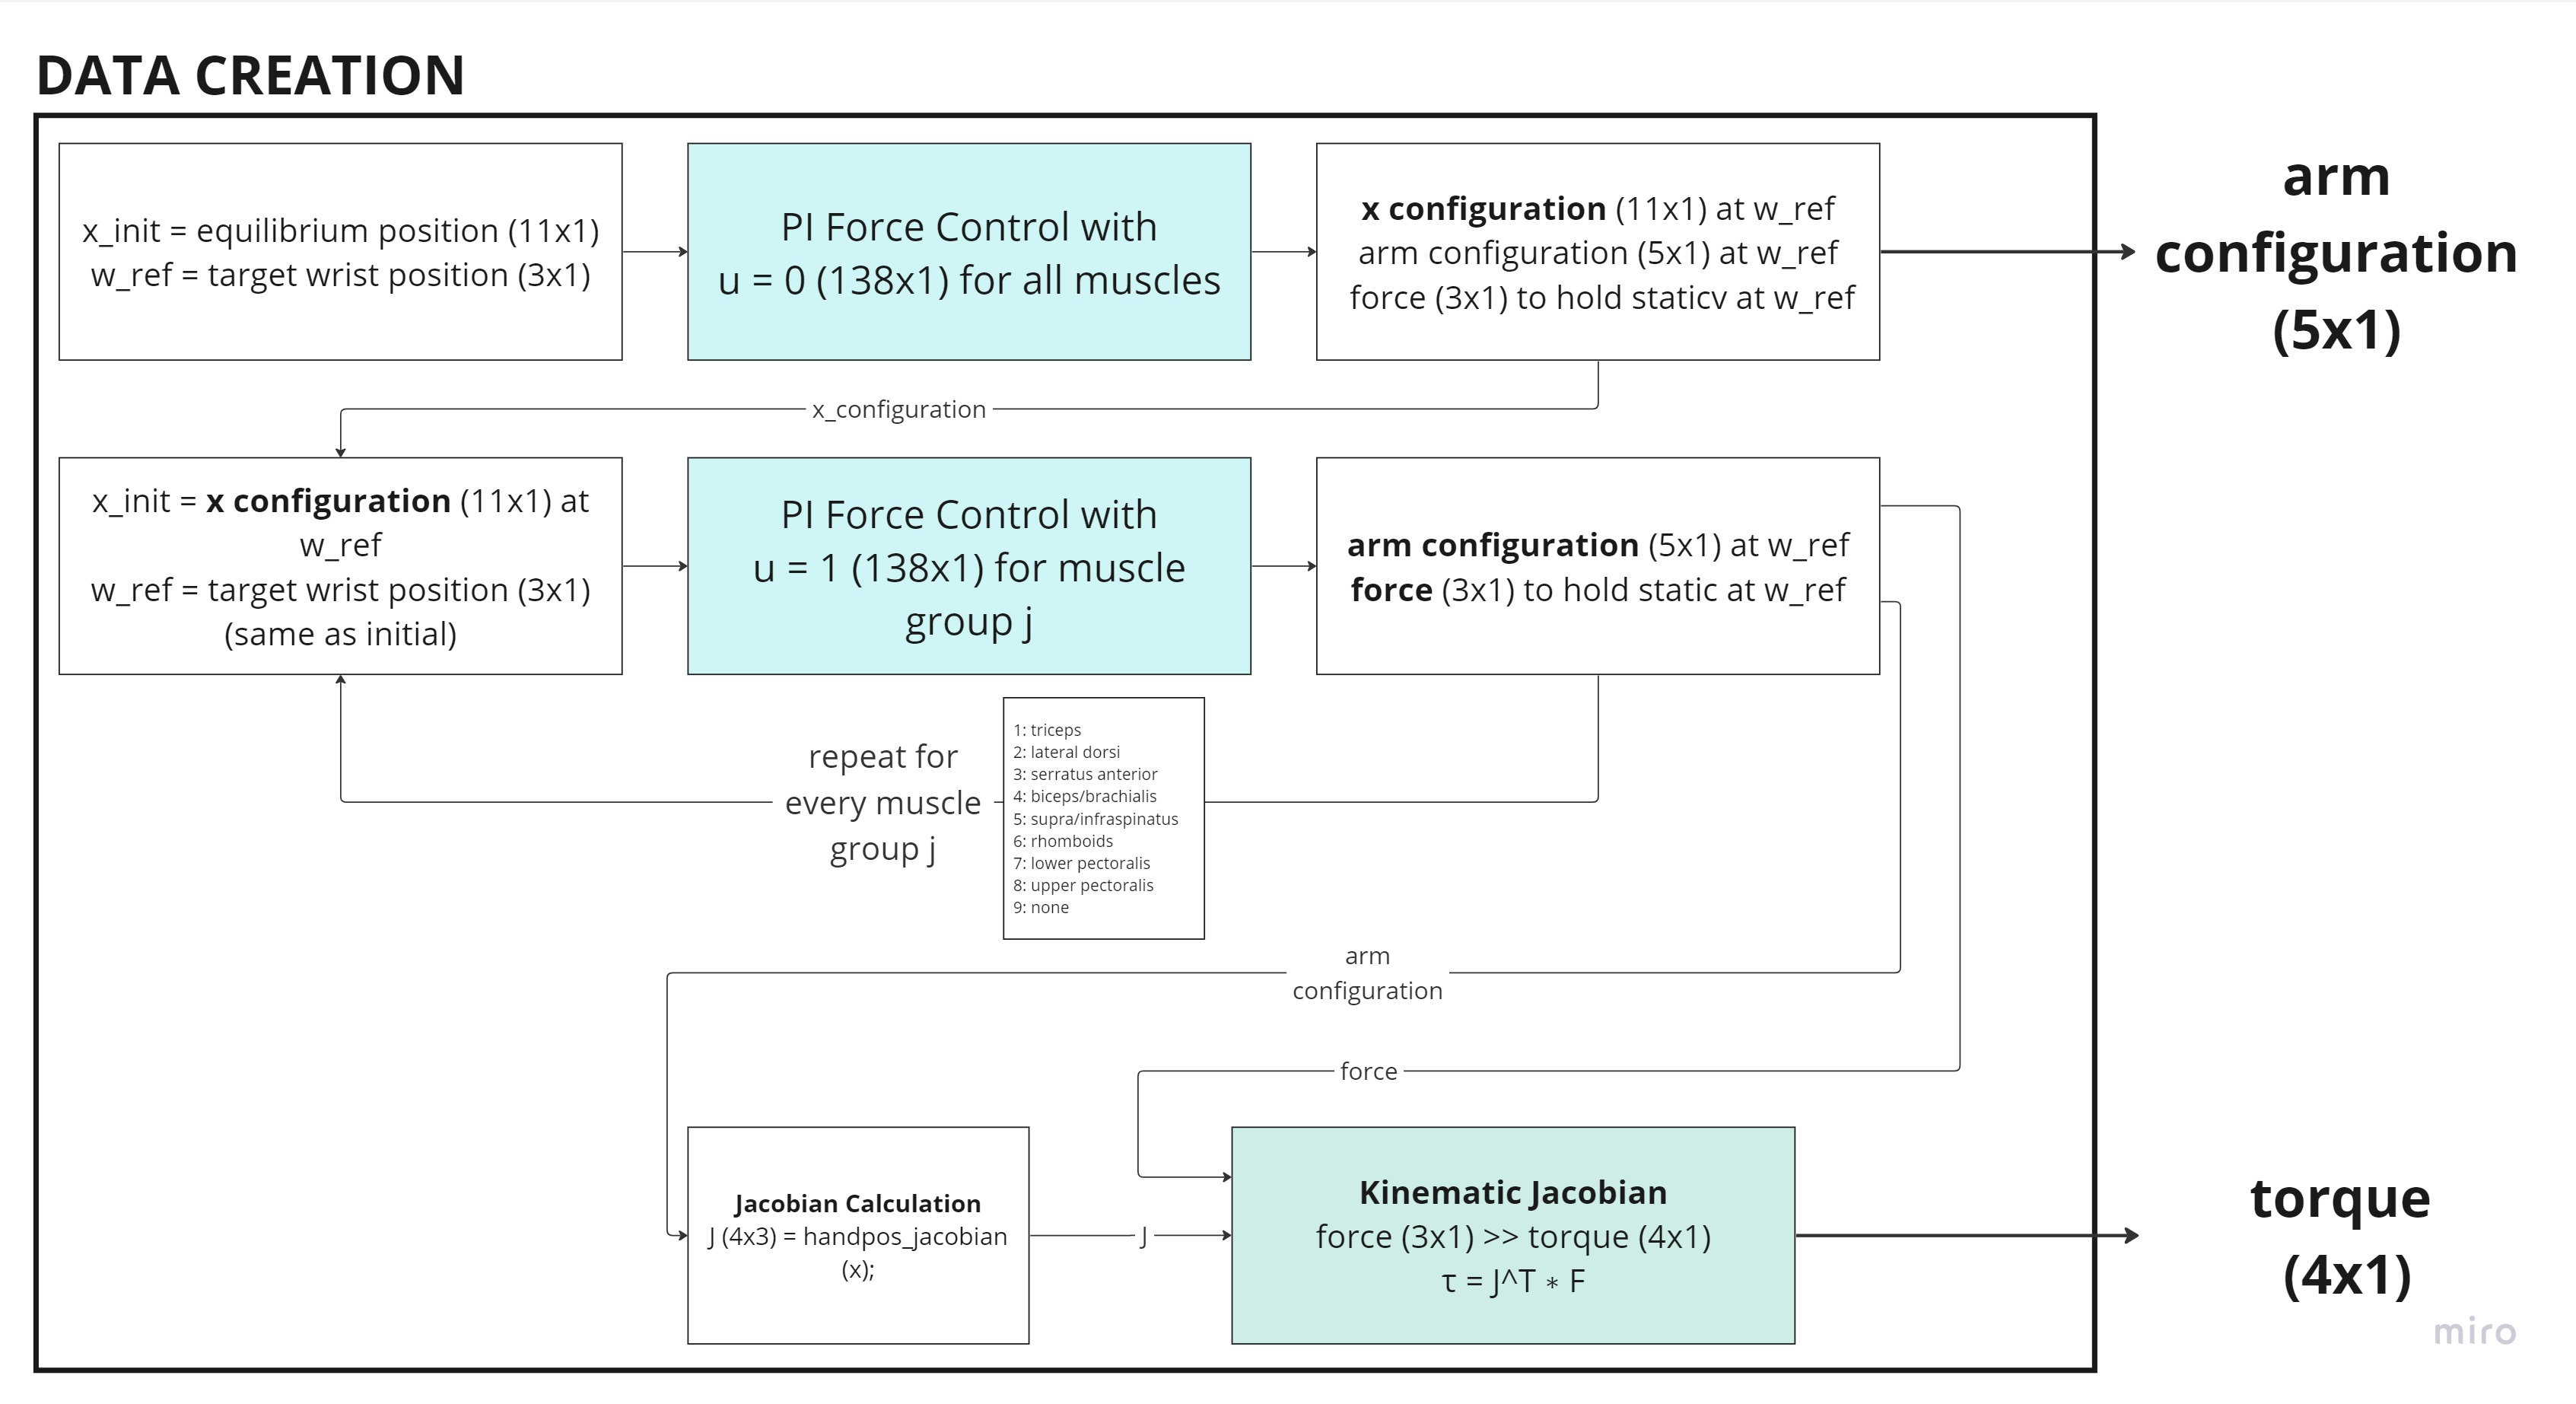
\includegraphics[width=1\textwidth]{Pictures/Model/DataCreation.jpg}
    \caption{Data Creation Flow Diagram}
    \label{fig:datacreation}
\end{figure}


Finally, the collected data is used to train the two semiparametric GPR models which are used to predict $\tau_j$ for a given configuration. The process is detailed in section \ref{sec:spgp} and a flow diagram is shown in Figure \ref{fig:modelcreation}.

\begin{figure}[h!]
    \centering
    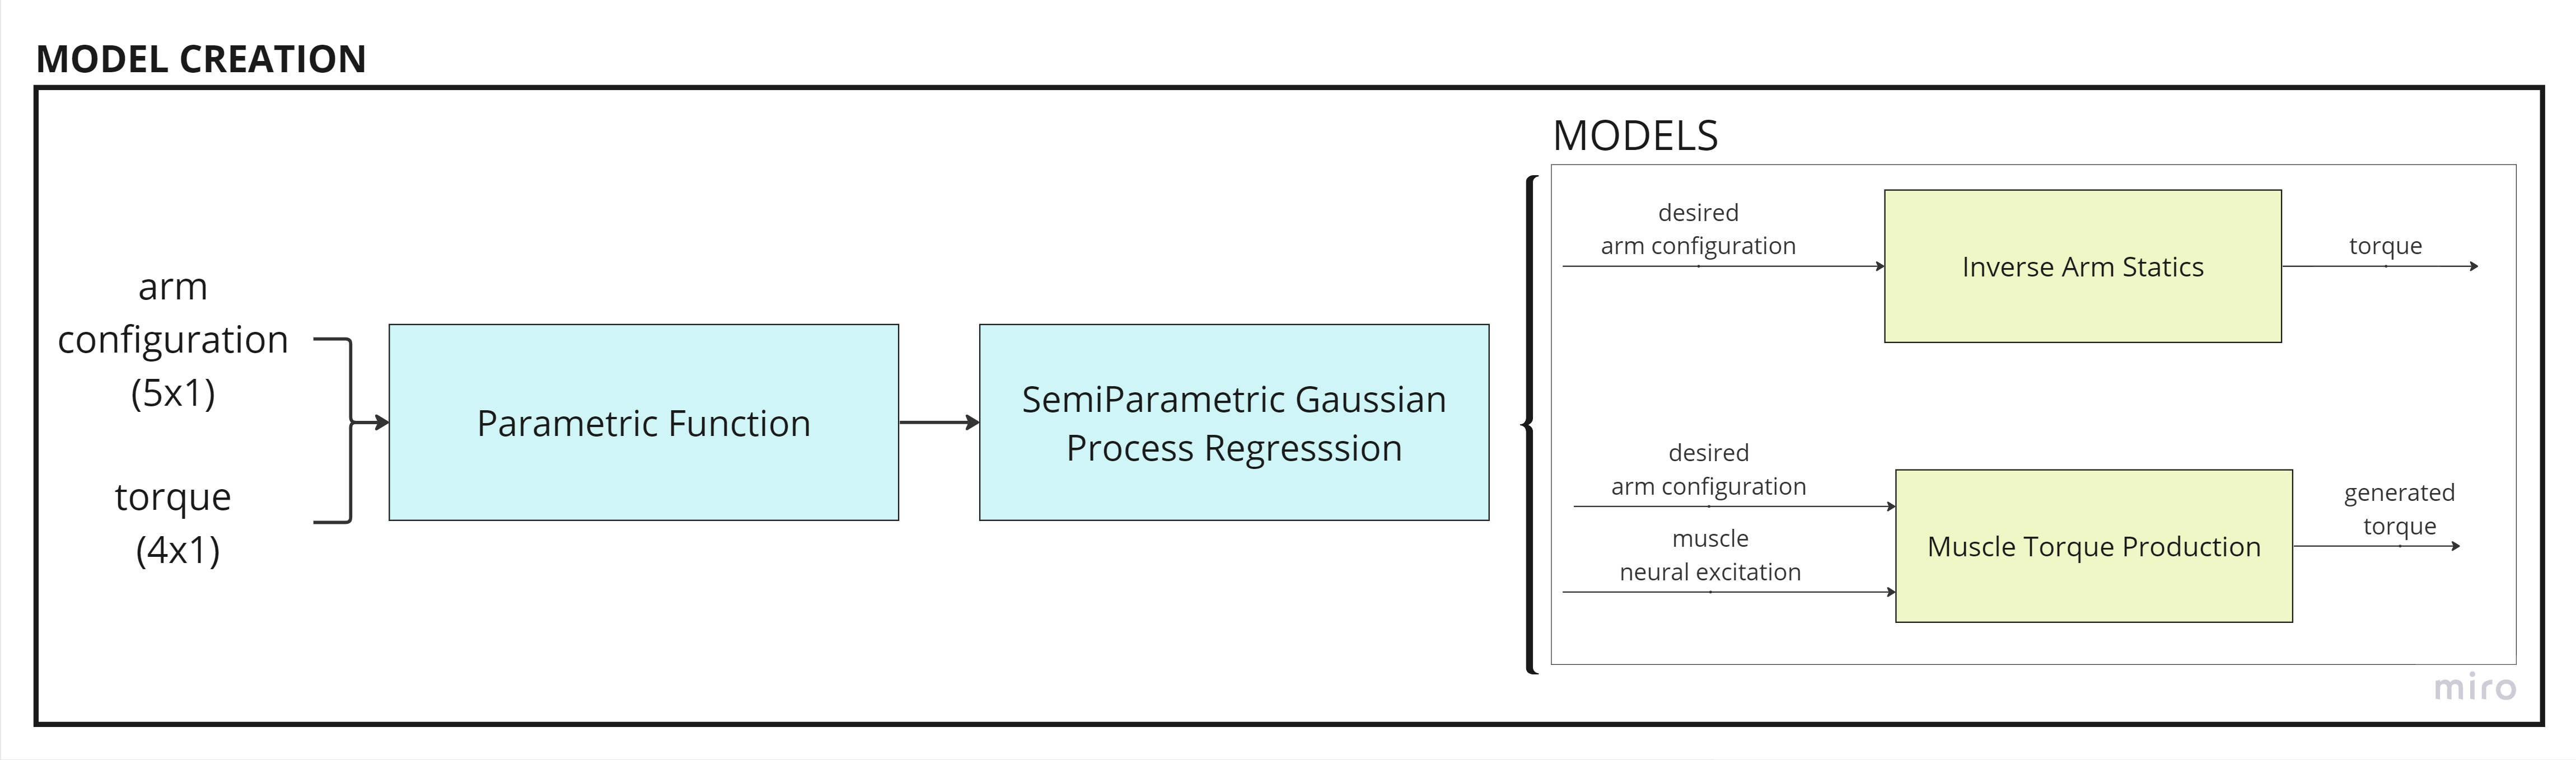
\includegraphics[width=1\textwidth]{Pictures/Model/ModelCreation.jpg}
    \caption{Model Creation Flow Diagram}
    \label{fig:modelcreation}
\end{figure}

 \section{Target Positions and Initial Configuration} \label{sec:tp}

 In the paper \cite{QSC} the simulated experiment resembles the one performed in a real-case scenario. A total of 27 different positions were analyzed where an external robot held the wrist of the arm into the different static positions. The robot was equipped with a three-dimensional force sensor at its end-effector \cite{HSAC}. 
 
 Since no real-world situation has been evaluated for this project, the simulation's goal is to represent a reaching motion beginning from an equilibrium posture. Additionally, the stroke survivor's arm is not being held by an external robot.As detailed in Section X, this approach stems from the assumption that the stroke survivor retains a degree of arm stability, sufficient to facilitate a limited reaching movement.  

 For this, it is decided to find calculate the forces in 64 different positions. This 64 positions are automatically generated using the function \textit{\textbf{create\_grid()}}.


The \textbf{\textit{create\_grid()}} function generates a grid of target points by defining the starting and ending coordinates for the x, y, and z dimensions and then linearly spacing these coordinates. If a model is provided as an input, the function also plots the wrist references, offering a visual representation of these coordinates.

\begin{table}[h]
    \centering
    \caption{Start and End Positions for x, y, and z Coordinates}

    \begin{tabular}{|c|c|c|}
        \hline
        Coordinate & Start Position & End Position \\
        \hline
        x & 0.3 & -0.08 \\
        y & 0 & -0.3 \\
        z & -0.1 & -0.35 \\
        \hline
    \end{tabular}
    \label{table:coordinates}
\end{table}

\begin{figure}[h!]
    \centering
    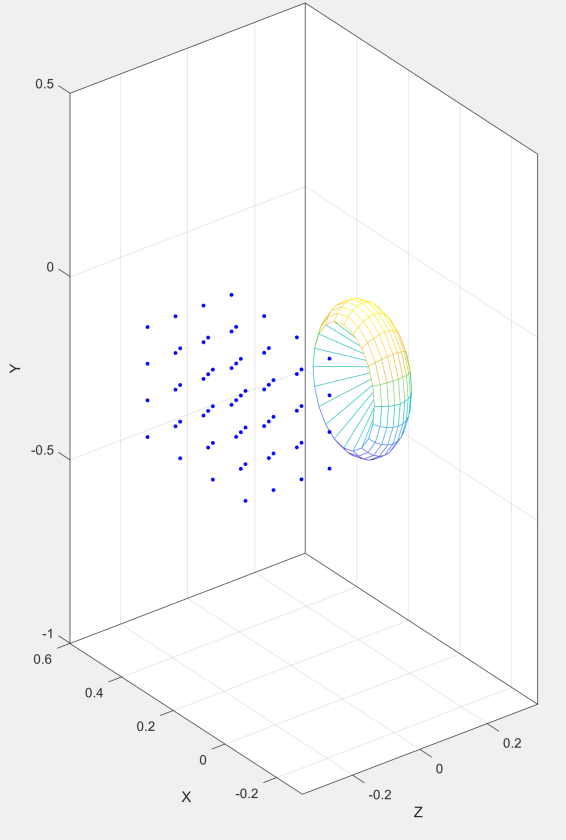
\includegraphics[width=0.4\textwidth]{Pictures/Model/create_grid.png}
    \caption{\textit{create\_grid} function output. 64 target positions used to calculate the required force to hold a this reference static positions with and without neural excitation.}
    \label{fig:create_grid}
\end{figure}

\newpage
\section{PI Force Controller}\label{sec:PI}

 The goal of the static force simulation is to determine the necessary force to keep the wrist in a specific static position. It involves two distinct scenarios. Both scenarios use a PI controller to exert the required force at the wrist, using the input \textit{handF} in the \textbf{\textit{das3\_step(...)}} function.

\begin{figure}[h!]
    \centering
    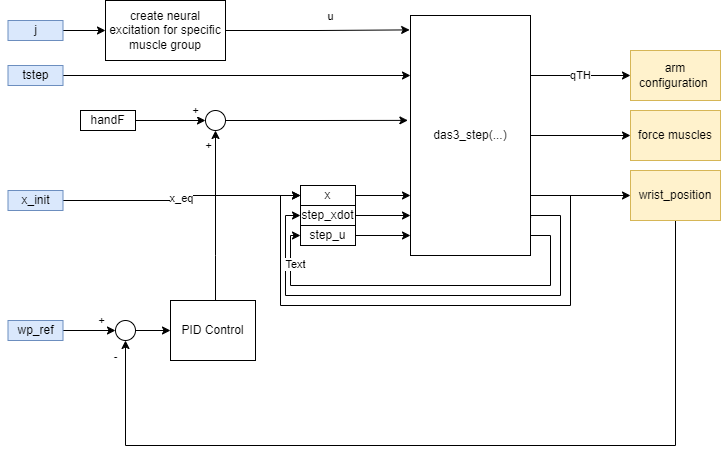
\includegraphics[width=0.9\textwidth]{Pictures/Model/PIController.png}
    \caption{Block Diagram for PI Force Controller}
    \label{fig:PIBlockDiagram}
\end{figure}

In the first scenario, no muscles are excited. The simulation starts from the equilibrium position and continues for 3 seconds, with a time step of 0.001 seconds. The focus is to calculate how much force is needed to apply to maintain a specific arm configuration static.

In the second scenario, the simulation begins with the arm configuration that was determined after running the previous no-excitation simulation. Here, one muscle at a time is stimulated at 100\%, i.e, $u_{j}$. The index j represents the muscle, this values goes from 1 to 9. Although the muscles may deviate from the starting position, the PI controller continuously adjusts to keep the hand in its initial position. This simulation is shorter, running for 0.5 seconds, but still utilizes a time step of 0.001 seconds.

After each time step,in both scenarios, the difference between the wrist's current position and the target is computed. This error is then multiplied by the Proportional (P) coefficient (Kp) of the PI controller. Concurrently, the accumulated error is updated and multiplied by the Integral (I) coefficient (Ki).  The sum of both the proportional and integral terms dictates the \textit{handF} for the next step (Equation \ref{eq:PID}). In the context of the PI controller, the proportional segment is responsible for creating an output in direct relation to the present error, while the integral portion systematically reduces  steady-state error by considering the history of past errors.

\begin{equation} \label{eq:PID}
\begin{aligned}
        error_{pos} = hand_{goal} - hand_{current}; \\
        error_{i} = error_i + error_{pos}*t_{step}; \\
        hand_F = K_p*error_{pos} + K_i*error_i; \\
\end{aligned}
\end{equation}
where $error_{pos}$ is the difference between the target goal and the current position, the $error_i$ represent the cumulative error from every time step and $hand_F$ is the calculated force that will be exerted on the hand to achieve the goal position.

The specific values for T, $t_{step}$, PI parameters for both scenarios are detailed in Table \ref{tab:PI}.

The force necessary to reach each point is calculated by averaging the last 10\% of the data collected during the simulation.The resulting information, including the forces exerted, mean force, and the arm's configuration, is  saved for each point in the simulation.

\begin{table}[h]
    \centering
    \caption{Values for Period (T), Time step ($t_step$), and PI Gains for PI controller with no neural excitation ($u_j=0$) and with neural excitation for each muscle ($u_j = 1$). The index j represents each muscle $j \epsilon[1,9]$.}
    \begin{tabular}{|l|c|c|}
        \hline
        \textbf{Parameter} & \textbf{$u_j=0$} & \textbf{$u_j=1$} \\
        \(T\) (Period) & 3 & 0.5 \\
        \(t_{step}\) (Time Step) & 0.001 & 0.001 \\
        \( K_p \) (Proportional Gain) & 2000 & 2000\\
        \( K_i \) (Integral Gain)     & 100 & 100 \\
        \hline
    \end{tabular}

    \label{tab:PI}
\end{table}

Below is a MATLAB code snippet that demonstrates the calculation of PI force, inclusive of the step simulation.

\begin{lstlisting}[style=Matlab-editor]
hand_current = wrist_position(x)
error_pos = hand_goal - hand_current
error_int = error_int + error_pos*tstep;

% PI calculation for time step
handF = K*error_pos+I*error_int;

[x, xdot, step_u] = das3step(x, u, tstep, xdot, step_u, M, exF, handF);
\end{lstlisting}

The function \textbf{\textit{wrist\_position(x)}} calculates the global position of the wrist using transformation techniques. Initially, the \textit{das3('Visualization',..)} is wrist position vector ($p$) and the orientation matrix ($R$). Constants and position vectors are defined, including the local coordinates of bone points.

Next, the function transforms the local coordinates into global ones. By utilizing the orientation matrix $\textbf{R}$ and the position vector $\textbf{p}$, it applies a transformation to the local coordinates, yielding the global coordinates \textbf{x}, \textbf{y}, and \textbf{z}. The process is a straightforward application of the principles of rotation and translation, aligning the local wrist coordinates with a global frame of reference.

\begin{equation}
\begin{aligned}
    p_{rotated} = R*p_{local} \\
    p_{global} = p_{rotated} + t
\end{aligned}
\end{equation}

where $p_{rotated}$ is the rotated position vector, $R$ is the orientation matrix, $p_{local}$ is the local position vector, and $t$ is the translation vector representing the shift from the local to the global coordinate system.


\newpage
\section{Kinematic Jacobian and Torque Calculation} \label{sec:torque} 

\subsection{Background} 

The Kinematic Jacobian is a critical part of the transformation of the recorded robot controller force to the joint torque $\tau_j$. The index j represents the muscle group being activated, when no muscle is being activated j is equal to 0.

In robotics, the Jacobian matrix provides essential information about the relationship between the velocities of the joints and the end-effector of a robot manipulator. This relationship can be expressed using the equation

\begin{equation}
\dot{x} = J \cdot \dot{q}
\end{equation}

where $\dot{x}$ is the end-effector velocity and $\dot{q}$ is the joint velocity.

Understanding the relationship between how the robot joint's velocities correlate to the end-effector's velocities is vital for planning trajectories in different spaces.

Furthermore, the kinematic Jacobian can be use to determined the necessary forces in joint space to achieve specific forces in end-effector space. In the musculosketal system it is assumed that the 11 degrees-of-freedom have no friction at the joint. The joint torques ($ \tau \epsilon R^n$) required to bear an endpoint/hand force ($F \epsilon R^{6x1}$), are given by,

\begin{equation}
    \tau = J^T*F
\end{equation}

where the Jacobian matrix ($J \epsilon R^{6xn}$) relates the infinitesimal joint displacement $dq$ to the infinitesimal end-effector displacements $dp$. The theorem is proven using the Principle of Virtual Work \cite{ITR}.

\begin{equation}\label{eq:displacement}
    dq = J*dp
\end{equation} 

Calculating the kinematic Jacobian in robotics involves defining the structure and parameters of the robot's joints and links, often using conventions like Denavit-Hartenberg (D-H) parameters. Transformation matrices are found for each joint, and the end-effector position is obtained by multiplying these matrices.

The Jacobian matrix is then constructed by differentiating the end-effector's position with respect to each joint variable, considering whether the joint is revolute or prismatic. The resulting 6×n matrix, where n is the number of joints, maps the joint velocities to the linear and angular velocities of the end-effector.

\subsection{Implementation}
The equation \ref{eq:displacement} is applied as shown in the MATLAB code below to calculate the torque values from the mean forces previously calculate using the PI controller. 

\begin{lstlisting} [style=Matlab-editor]
[dPhand_dx, ~, ~] = handpos_jacobian(x);
torque = dPhand_dx'*hand_F;
\end{lstlisting}

Due to the complex system, to calculate the kinematic Jacobian of the arm, the concept of infinitesimal displacement presented in Equation \ref{eq:displacement} is used. The function \textbf{\textit{handpos\_jacobian(x)}} (MATLAB code below) take the state and perturbs each degree of freedom by a small mount $h$. For each perturbation, the old and the new hand positions are  subtracted and divided by $h$. This describes how the changes in the degrees of freedom affect the hand´s position at that particular state. 

\begin{lstlisting}[style=Matlab-editor]
function [dPhand_dx, Phand, Phand_new] = handpos_jacobian(x)
    dPhand_dx = zeros(3,11);
    stick = das3('Visualization', x);
    Phand = stick(13,1:3)';
    h = 1e-7;
    for i = 1:11
        tmp = x(i);
        x(i) = x(i) + h;
        stick = das3('Visualization',x);
        Phand_new = stick(13,1:3)';
        dPhand_dx(:,i) = (Phand_new - Phand)/h;
        x(i) = tmp;
    end        
end
\end{lstlisting}

The shoulder and elbow torques are computed using the transpose of the kinematic Jacobian. They are denoted by $\tau_{j}$, where $j$ symbolizes the muscle group being activated, with 0 signifying no active muscles. The torque concerning elbow pronation is disregarded as it does not influence the wrist's positions. 

If no muscles are activated, the torque needed to hold the the wrist in static position is equal to,

\begin{equation}
\tau_0 = p(q)
\end{equation}

where $p(q) \epsilon  R^{4x1}$. 

The torque produced by the muscle's group $j$ activations is calculating by subtracting the torques recorded when no muscles are activated and the torques recorded with muscle group $j$ active. This torque  is represented by $M(q)\alpha$ where $\alpha \epsilon M^{8x1}$ is the vector of muscle group activations and $M(q) \epsilon M^{4x8}$ is the mapping from muscle group activation to joint torque. It is assumed that the torques scales linearly with activation \cite{SPI}. 

\begin{equation} \label{eq:MAP}
    M_j(q) = \tau_0 - \tau_j
\end{equation}

Each column of $M(q)$ describes the torque generated by each muscle group at full activation. It is assumed that individual muscle torques add linearly without interference from adjacent muscles or connective tissue interactions. 




\newpage
\section{Model Creation: Semi-Parametric Gaussian Process Regression} \label{sec:spgp}

\subsection{Comparative Analysis of Model Types}

A comparative accuracy analysis was conducted between non-parametric, semiparametric, and parametric models in \cite{SPI}. The semiparametric GP model resulted as the most accurate, combining the flexibility of a black-box function approximation with the generalization strength of a parameterized model, as indicated in \cite{SPI}. This semiparametric model estimated torques during muscle stimulation with less than 20\% error relative to the total muscle torque and passive torque required to move the arm. 

Details on the quality of the model can be found in \cite{SPI}. A summary of the three models is described in the table \ref{table:comparison}.


\begin{table}[ht]
\centering
\begin{tabularx}{\textwidth}{|c|X|X|X|}
\hline
\multirow{6}{*} & \textbf{Description} & \textbf{Advantages} & \textbf{Disadvantages} \\
\hline
\multirow{5}{*}{\rotatebox{90}{\textbf{Parametric}}} & Linear model used to represent torque in a single degree of freedom, accounting mainly for joint stiffness and damping. & Simplicity and efficiency due to linear nature. It avoids solving nonlinear optimization problems. & Inaccuracy with full complexity. Limited application in simpler version as it does not account for physicial properties. \\
\hline
\multirow{7}{*}{\rotatebox{90}{\textbf{Nonparametric}}} & Utilizes Gaussian process regression to predict arm joint torques, defining mean and covariance functions. It relies on training samples to make predictions. & Adaptability, less overfitting, avoids identifiability issues as it does not need rich enough data to guarantee identifiability of parameters. & Computational complexity and demanding. \\
\hline
\multirow{13}{*}{\rotatebox{90}{\textbf{Semiparametric}}} & Combines aspects of both parametric and nonparametric models. It uses a Gaussian process where the mean function is derived from the parametric model and the covariance is the sum of a squared-exponential covariance function and an term for uncertainty in the parameters of the parametric model. & Flexibility, generalization, local relevance (dominate predictions for inputs close to training data) with complex dynamics. & Complexity in understanding, implementing, and tuning. \\
\hline
\end{tabularx}
\caption{Comparison of Parametric, Nonparametric, and Semiparametric Models}
\label{table:comparison}
\end{table}

\subsection{Background}

Gaussian Process Regression (GPR) is a powerful and flexible tool used in machine learning for fitting a function to data. It is rooted in the mathematical foundation of Multivariate Gaussian Distributions, where each random variable is distributed normally, and their joint distribution is also Gaussian. GPR can be expressed as 
\begin{equation}
    f(x) \sim \mathcal{GP}(\mu(x), k(x, x'))
\end{equation}
where  \( \mu \) is the the mean vector and \( k(x, x') \) is the covariance or kernel function. The mean vector \( \mu \) describes the expected value of the distribution, while the kernel models the variance along each dimension and determines how the different random variables are correlated. The covariance matrix is always symmetric and positive semi-definite.

GPR creates a model of the function it is trying to learn, using a process that considers an infinite number of dimensions and includes an element of randomness. It encapsulated initial beliefs about the function in the \textit{prior distribution}, defined by the mean and kernel functions. Observations are used to update these beliefs through the \textit{likelihood function}, leading to the computation of the \textit{posterior distribution}. This posterior reflects updated beliefs about the possible functions that best fit the data.

Predictions are made by calculating the mean and variance of the predictive distribution at new inputs, allowing for both point estimates and uncertainty estimates. 

In summary, GPR operates on the foundational principles of Bayesian inference to model a function from given data. This enables GPR to deliver both point predictions and associated uncertainties. The inherent flexibility and adaptability of GPR make it a powerful and widely applicable tool for function approximation in machine learning and statistical analysis. \cite{GPR}

\begin{figure}[h!]
    \centering
    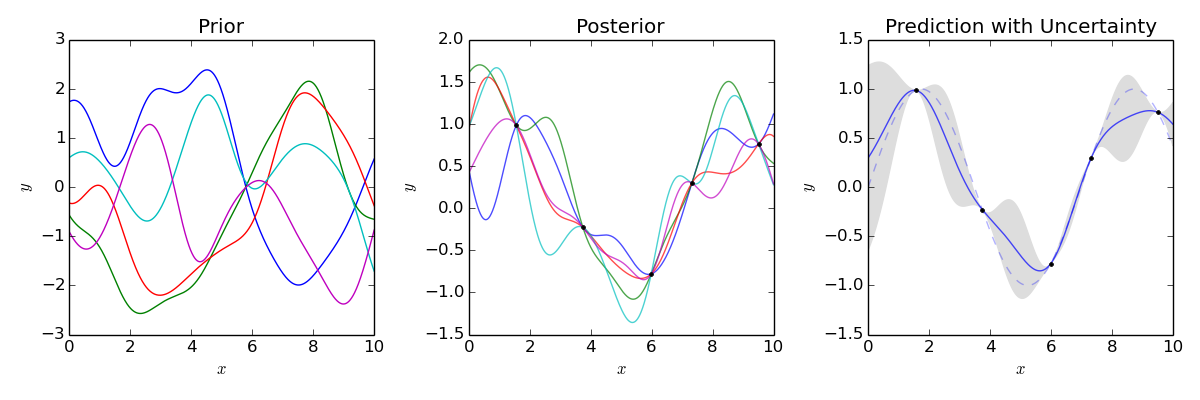
\includegraphics[width=0.9\textwidth]{Pictures/Model/Gaussian_Process_Regression.png}
    \caption{Gaussian Process Regression \cite{GPR_Image}}
    \label{fig:GPR}
\end{figure}





\subsection{Implementation}

Based on the results of the aforementioned study, the data for the set of 64 training positions is used to train semiparametric GPR models which are used to predict $\tau_j$ for a given configuration. The models are used to determine the static arm torques $p(q)$ and the muscle force mapping $R(q)$ for a desired arm configuration.
The kernel function used in the GPR was the squared exponential function using the distance metric for rigid bodies. 
 
A MATLAB script, \textbf{\textit{compute\_GPR\_model}}, is designed to compute the model performing Gaussian Process Regression to fit the data. This code loads the data and does GPR for each muscle where the inputs are the arm configuration angles and the output are the joint torques.

The flow diagram shows the steps of the code.

A more thorough description is presented below.

After initializing the prior parameters and the covariance matrices the data containing the information related to each model is loaded. The script sets up 10 specific muscles and 64 target positions. 

A loop iterates through each muscle, fexecuting the following steps:

\begin{itemize}
    \item \textbf{Data Extraction}. The angle and torque data to each muscle is extracted.
    \item \textbf{Model Fitting} The script applies both parametric and semiparametric fitting methods to the five different configurations: elevation plane, shoulder elevation, shoulder rotation, elbow flexion and elbow pronation. Custom function \textbf{\textit{parametricfunctionReach}} and \textbf{\textit{semiparametricfunctionReach}} are called to perform the fitting process. These functions incorporate GPR to build models that capture the underlying relationship between joint angles and torques.
    \item \textbf{\textit{Output Model}}. Once the analysis is completed the \textbf{modeldata} structure containing the details of the models for all muscles is saved into a MATLAB file. 
\end{itemize}

\textbf{\textit{PARAMETRIC FUNCTION}}

For the \textbf{parametricfunctionReach}, Bayesian Regression (\cite{BLM}) is used to calculate the mean ($\mu$) and the covariance ($\Sigma$) for the prior parameter distribution for the semiparametric model. Bayessian Regression is a statistical method that estimates the unknown parameters of a linear model by considering them as random variables with prior distributions. It takes into account prior knowledge of the parameters to provide a more precise understanding.

In the following paragraphs, the code and the corresponding mathematical implications will be detailed.  Refer to figure \ref{fig:ModelComputationGPR} for a detailed flow diagram.

First the basis function or design matrix ,$\Phi$, is evaluated for each arm configuration torque. It is used to represent the relationship between the input variables and the target outputs in a compact and mathematical form. 

Then a residual squared error computation following Equation \ref{eq:rsq} is calculated , where the model parameter, $\beta$, to predict the outputs is calculated by isolating it from the linear model. \( y \) is the target/output vector, \( \Phi \) is the design matrix, \( \beta \) is the vector of coefficients,\( \hat{y} \) is the predicted output vector and  \( sqres \) is the residual error. This residual error will act as the covariance matrix noise.

\begin{equation}
\begin{aligned}
    y = \Phi \beta \\
    \beta = \Phi^+y \\
    \hat{y} = \Phi*\beta \\
    sqres = mean((\hat{y}-y)^2) \\
\end{aligned}
\end{equation} \label{eq:rsq}

Finally, the mean \( \mu \) and covariance \( \Sigma \) of the parameter $\beta$ distribution  that will define the prior distribution for the semiparametric model are calculated as a posterior distribution following the Bayesian linear regression.  

The prior distribution mean \( \mu_0 \) and covariance \( \Sigma_0 \) are given as input to the function. A Gaussian prior distribution describes the parameters \( \beta \) distribution.
\begin{equation}
  p(\beta) = \mathcal{N}(\beta | \mu_0, \Sigma_0)
\end{equation}
where \( \mu_0 \) is the prior mean, and \( \Sigma_0 \) is the prior covariance matrix.

Given the data, the distribution is updated using Bayes' theorem to find the posterior distribution over the parameters:
\begin{equation}
    p(\beta | \Phi, y) \propto p(y | \Phi, \beta) \cdot p(\beta)
\end{equation}

Assuming Gaussian noise, the likelihood term is also Gaussian:
\begin{equation}
  p(y | \Phi, \beta) = \mathcal{N}(y | \Phi \beta, S)
\end{equation}
where \( S \) is the covariance matrix of the noise.

The posterior distribution for \( \beta \) given \( y \) and \( \Phi \) is also Gaussian, and its mean \( \mu \) and covariance matrix \( \Sigma \) can be found as follows:

\begin{equation}
\begin{aligned}
     \mu = \Sigma (\Phi^T \Sigma^{-1} y + S_0^{-1} \mu_0) \\
    \Sigma = \left( \Sigma_0^{-1} + \Phi^T S^{-1} \Phi \right)^{-1}
\end{aligned}
\end{equation}

In summary, the prior mean \( \mu_0 \) and covariance \( \Sigma_0 \) encapsulate our beliefs about the coefficients before seeing the data. The design matrix \( \Phi \) and the response vector \( y \) represent the data we observe. The posterior mean \( \mu \) and covariance \( \Sigma \) encapsulate our updated beliefs about the coefficients after seeing the data.

\textbf{\textit{SEMI-PARAMETRIC FUNCTION}}

In the following paragraphs, the code and the corresponding mathematical implications will be detailed.  Refer to figure \ref{fig:ModelComputationGPR} for a detailed flow diagram.

First the basis function or design matrix ,$\Phi$, is evaluated for each arm configuration torque. It is used to represent the relationship between the input variables and the target outputs in a compact and mathematical form. 

A Gaussian Process is fully specified by the \textbf{mean function} and a \textbf{covariance function}. Following \cite{SPI}, the mean function is the parametric model and the covariance function is the sum of squared-exponential covariance (Equation \ref{seard})  function and a term that takes into account the uncertainty in the parameters of the parametric model. 
\begin{equation}
\begin{aligned}
    \mu = \Phi*\beta \\
    \Sigma = k(x,x')  + \Sigma_{uncertainty}
\end{aligned}
\end{equation}

\begin{equation}\label{seard}
    k(x,x') = \sigma^2*\exp{-\frac{(x-x')^2}{2l^2}}
\end{equation}

The length scale ($l$) were chosen a priori to be small which means that the correlation between observations drops off quickly as their separation increases. Leading to a more flexible model. 

The vertical scale ($\sigma^2$) controls the overall variance of the function values. Higher values means more significant variation from one point to another, allowing GP to capture strong fluctuations. 

Moreover the likelihood function chosen is the Gaussian Likelihood. The likelihood describes the noise model, in this case assuming normally distributed noise. 

Next, hyper-parameters GPR are defined. Hyperparameters are essential parameters that define how the model behaves. There are three main hyperparameters:

\begin{itemize}

    \item Mean. The mean previously calculated in the parametric function.
    \item Covariance. It includes, the length scale parameters, the vertical scale hyperparameters and the covariance previously calculated in the parametric function. 

    \item Likelihood function. It is set to be the $log(10)$ which suggests a specific setting on the noise variance in the Gaussian likelihood. 

\end{itemize}

The hyperparameters are optimized to the GP model to best explain the training data. The optimized hyperparameters are used to make predictions using Gaussian Process model. All Gaussian process computations are made using the GPML toolbox for MATLAB (\cite{GPML}).

\begin{lstlisting} [style=Matlab-editor]
covGP = {@covSEard};
likfunc = @likGauss;
covfunc1 = {'covSum',{covGP,covUNCERT}};

% optimize the hyperparameters and then make predictions with the optimized
% parameters
[hypOPT fX iter] = minimize(hyp1, @gp, -100, @infExact, meanfunc1, covfunc1, likfunc, trainingInputs, trainingOutputs(:,1));
[meantest covtest] = gp(hypOPT, @infExact, meanfunc1, covfunc1, likfunc, trainingInputs, trainingOutputs(:,1), testInputs);
%prediction: [ymu ys2 fmu fs2   ] = gp(hyp, inf, mean, cov, lik, x, y, xs);
\end{lstlisting}

The prediction outputs are $y_{mu}$ (meantest) for test output mean and $y_{s2}$ (covtest) for test output covariance. 

The output of the semiparametric model are the \textbf{hyperparameters} that will be used later for future predictions.

\newpage
\begin{landscape} % Start landscape page
  \begin{figure}[h!]
    \centering
    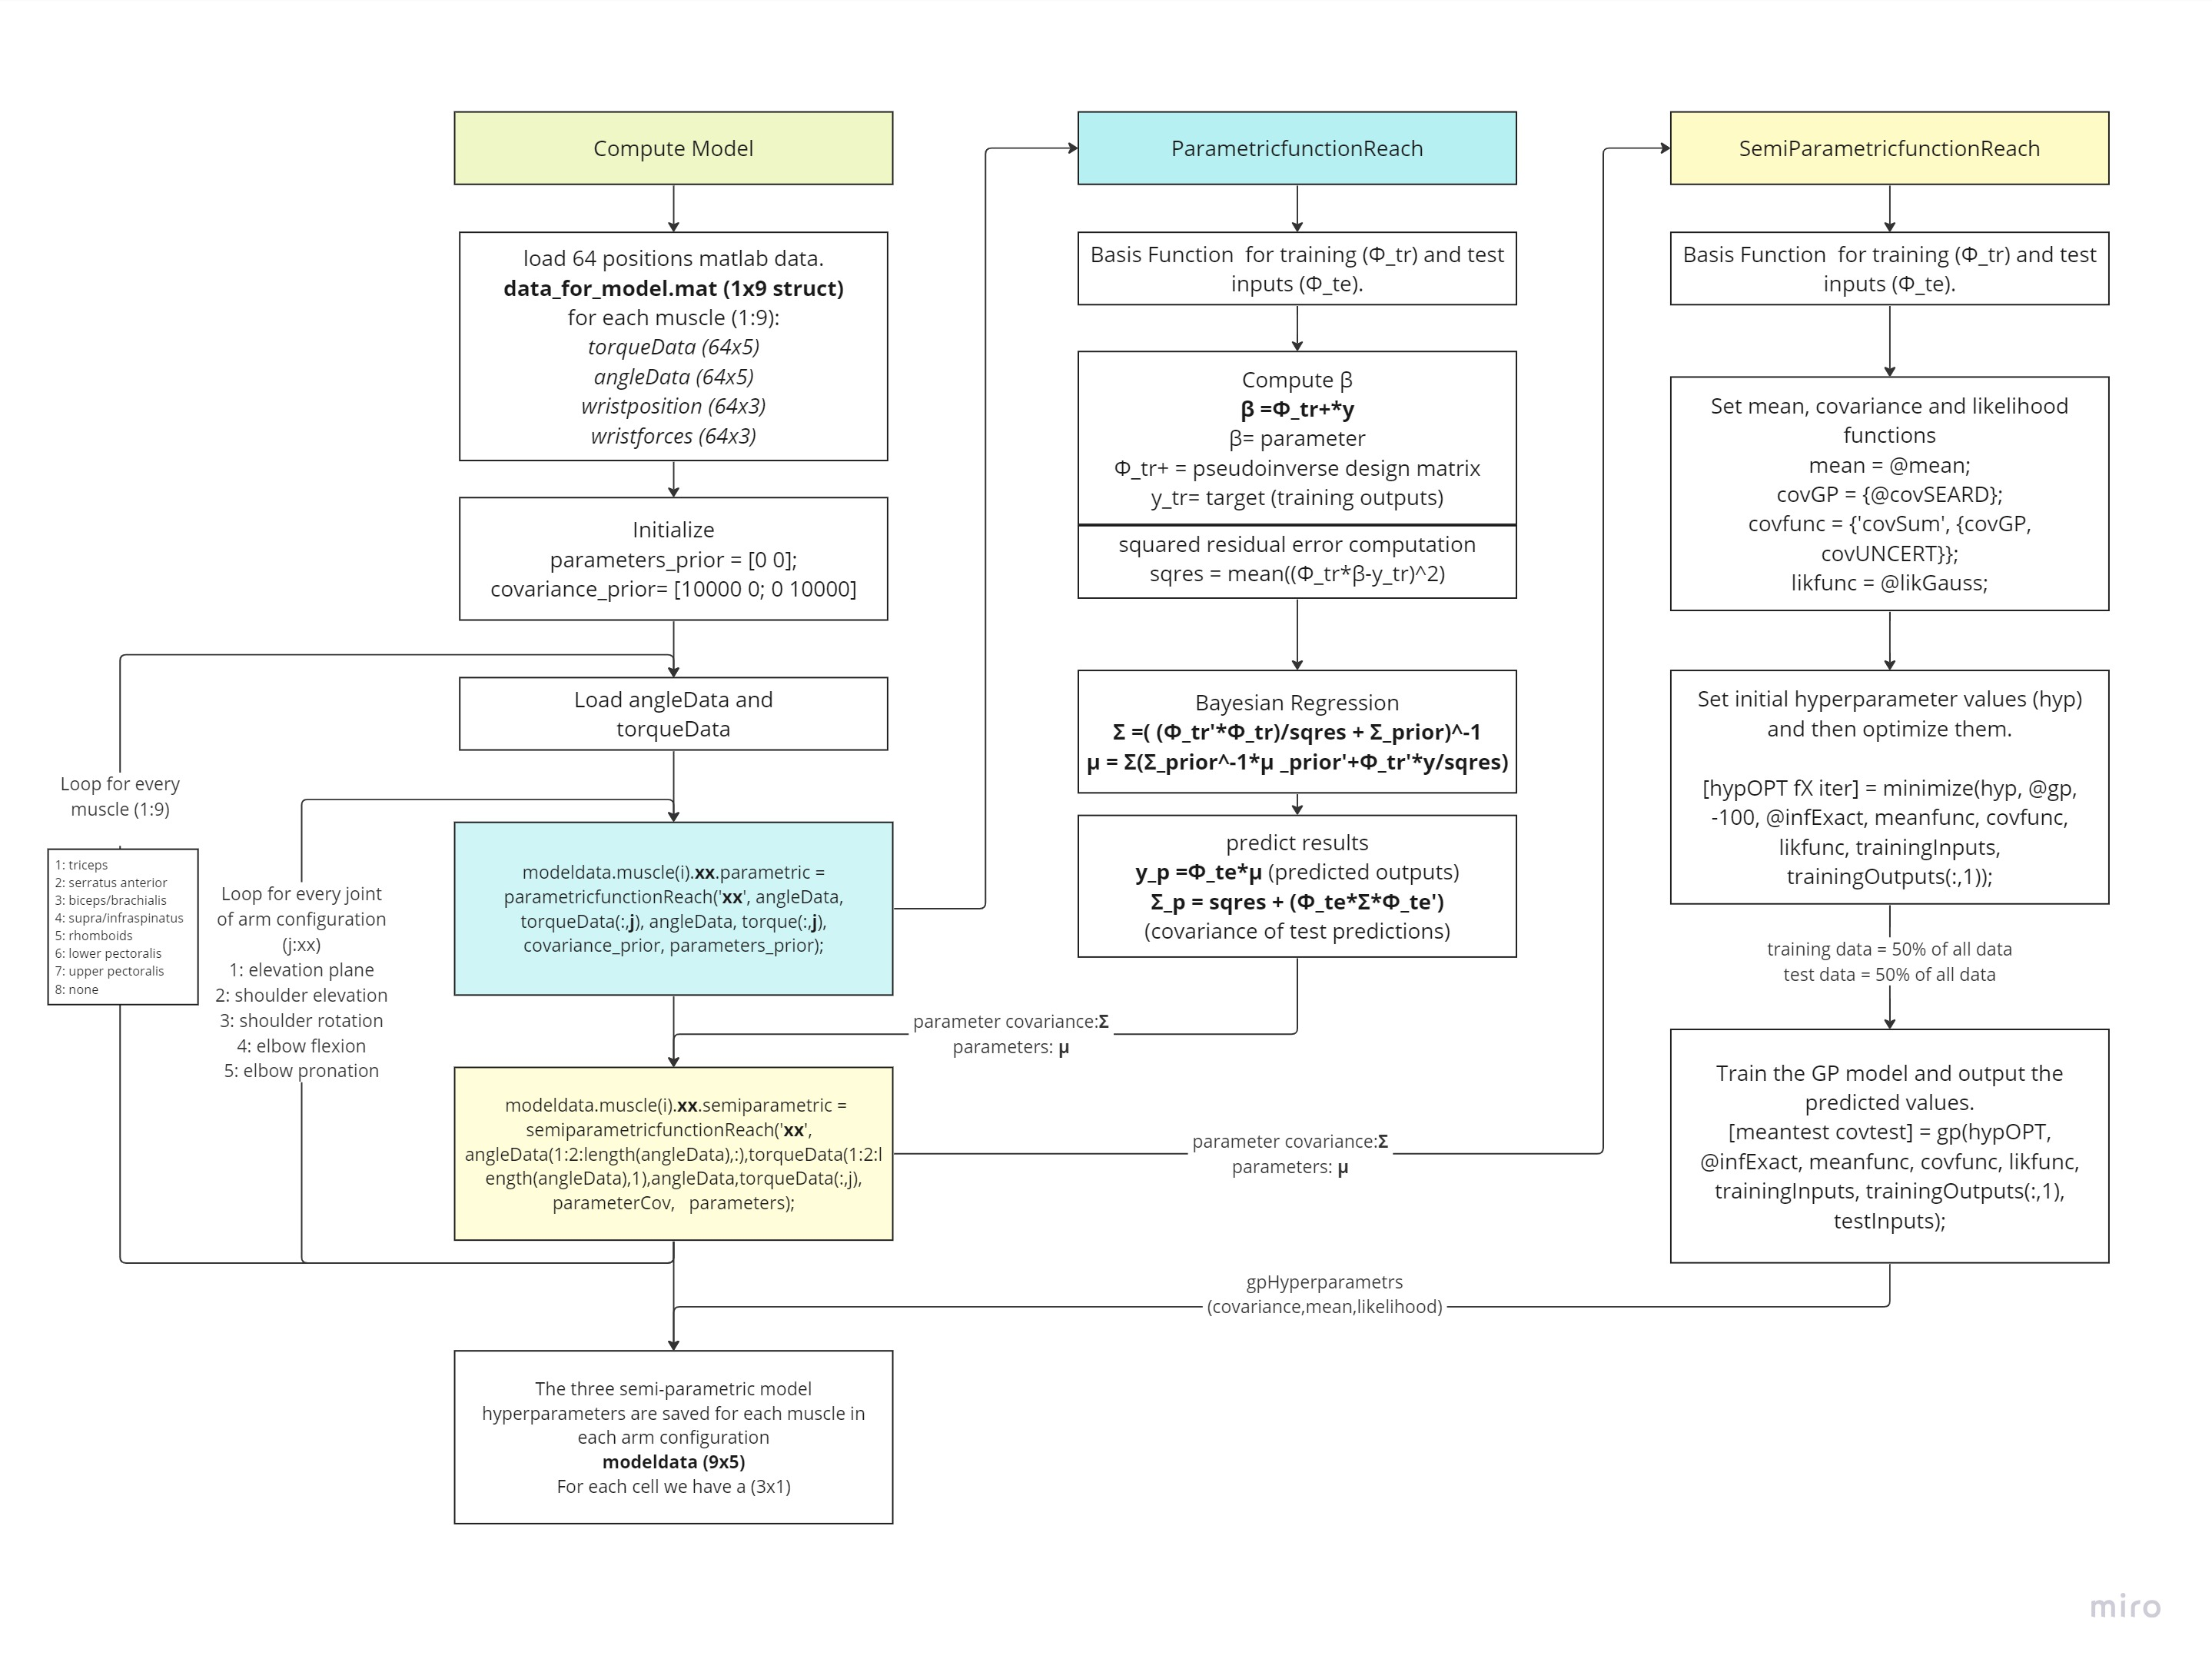
\includegraphics[width=1.4\textwidth]{Pictures/Model/computemodel.png} % Replace "filename.jpg" with the name of your image file
    \caption{Flow Diagram for Model Computation of Semi-Parametric GPR} % Optional caption
    \label{fig:ModelComputationGPR} % Optional label for referencing
  \end{figure}
\end{landscape} % End landscape page

